%%%%%%%%%%%%%%%%%%%%%%%%%%  phdsymp_sample2e.tex %%%%%%%%%%%%%%%%%%%%%%%%%%%%%%
%% changes for phdsymp.cls marked with !PN
%% except all occ. of phdsymp.sty changed phdsymp.cls
%%%%%%%%%%                                                       %%%%%%%%%%%%%
%%%%%%%%%%    More information: see the header of phdsymp.cls   %%%%%%%%%%%%%
%%%%%%%%%%                                                       %%%%%%%%%%%%%
%%%%%%%%%%%%%%%%%%%%%%%%%%%%%%%%%%%%%%%%%%%%%%%%%%%%%%%%%%%%%%%%%%%%%%%%%%%%%%%


%\documentclass[10pt]{phdsymp} %!PN
%\documentclass[twocolumn]{phdsymp} %!PN
%\documentclass[12pt,draft]{phdsymp} %!PN
%\documentstyle[twocolumn]{phdsymp}
%\documentstyle[12pt,twoside,draft]{phdsymp}
%\documentstyle[9pt,twocolumn,technote,twoside]{phdsymp}
\documentclass[a4paper,oneside,12pt]{article}

\usepackage{pdfpages}
\usepackage{a4wide}
\usepackage[english]{babel} 
\usepackage{url}
\usepackage{caption}
\usepackage{multirow}
\usepackage{rotating}
\usepackage{soul}
 
\usepackage{palatino}

\usepackage{graphicx}
\graphicspath{{figures/}} 
\def\BibTeX{{\rm B\kern-.05em{\sc i\kern-.025em b}\kern-.08em
    T\kern-.1667em\lower.7ex\hbox{E}\kern-.125emX}}

\newtheorem{theorem}{Theorem}

% zet de paragrafen een beetje uit elkaar en links uitgelijnd
\setlength{\parindent}{0mm}
\setlength{\parskip}{1ex plus 0.5ex minus 0.2ex} 

\setlength{\textheight}{23cm}
\setlength{\textwidth}{16cm}
\setlength{\oddsidemargin}{0cm}
\setlength{\evensidemargin}{0cm}
\setlength{\topmargin}{-1cm}

\penalty-10000
\tolerance=10000

% \setlength{\parskip}{0pt}
% \setlength{\parsep}{0pt}
% \setlength{\headsep}{0pt}
% \setlength{\topskip}{0pt}
% \setlength{\topmargin}{0pt}
% \setlength{\topsep}{0pt}
% \setlength{\partopsep}{0pt}

\linespread{0.9725}

\usepackage[compact]{titlesec}
%\titlespacing{\section}{1pt}{*0}{*0}
%\titlespacing{\subsection}{1pt}{*0}{*0}
\titlespacing{\subsubsection}{1pt}{*0}{*0}

\usepackage{mdwlist}

\begin{document}


%-------------------------------------------------------------------------------------------

\thispagestyle{empty}

\begin{center}
\mbox{}\\\vspace{5mm}
{\Large Application for China Scholarship Council Grant}\\ [45mm]
%
{\bf\Huge Hardware acceleration for\\
[3mm] FPGA CAD Tools} \\
\vspace{45mm}
\Large Yun Zhou \\
\vspace{2mm}
\small\texttt{\hl{email@address.com}} \\
\vspace{20mm}
\Large Advisor: ir.\ Elias Vansteenkiste \\
\small\texttt{Elias.Vansteenkiste@ugent.be} \\
\vspace{2mm}
\Large Promotor: prof.\ dr.\ ir.\ Dirk Stroobandt \\
\small\texttt{Dirk.Stroobandt@ugent.be} \\
\vspace{20mm}
\normalsize Ghent University, Belgium \\
\normalsize Department of Electronics and Information Systems\\
\normalsize Computer Systems Lab\\
\normalsize Hardware and Embedded Systems Group 
\end{center}

\newpage

\tableofcontents

\clearpage

\section{Problem Definition \hl{(1 page)}}
A Field Programmable Gate Array (FPGA) is an integrated circuit made up of a grid of programmable functional blocks embedded in a programmable interconnection network. An FPGA can be programmed to implement any arbitrary logic function in the same way as Application Specific Integrated Circuits (ASICs), however the functionality of an FPGA is not fixed during the production process. The functionality can be changed by writing a different configuration to the configuration memory. This flexibility of FPGAs leads to a substantial reduction of the economic risk of developing hardware accelerators. It also explains the rise in the popularity of the FPGA. Unfortunately the flexibility of the FPGA comes at a price.  Each time the application developer wants to test his design, the design has to be compiled to a FPGA configuration and this is a complex and time consuming process. Unfortunately the designer typically needs to compile his application numerous times to test if his/her design meets the constraints of the application. 

The main FPGA device manufacturers and the academic community have developed a chain of heuristics to solve the NP hard problems involved in the compilation.
The compilation/translation of a high-level description of the application to a FPGA configuration is typically divided in several steps. In each step NP hard problems have to be solved and heuristics were and are being developed to try to approximate an optimal solution. The most time-consuming steps are the placement and routing steps. They are the last steps at the backend of the tool flow. These steps have to performed to obtain accurate timing information, which is needed to assess if the design meets the constraints. 
 
Another trend is the increase in both the size of applications and the size of the target devices. FPGA device and application sizes are still increasing following Moore's law~\cite{shannon2015technology}. Unfortunately the power of the FPGA CAD tools lag behind. The traditional CAD heuristics scale very badly in terms of application and device size, which translates to waiting times of hours up until days for compilation to finish \cite{murray2015timing}. 

Since the introduction of high-level synthesis\cite{}, more and more engineers with a software background attempt to accelerate applications with an FPGA. They are used to gcc-like compilation times. Their design methodologies are adapted to these short compilation times. In order to fix bugs and measure performance the compilation is performed numerous times. Hence, they cannot accept the long compilation times that are common in FPGA design.

To overcome this problem, device manufacturers and academics developed multi-threaded versions of the heuristic algorithms \cite{ludwin2011,gort2012,betz2013method,jain2014multi}, but unfortunately scalability issues still exist and large designs still need hours to be compiled. To further speed up compilation a straightforward path is to use hardware acceleration, but unfortunately the current multi-threaded algorithms for placement and routing are hard to adapt for the wide scale parallelisation used in hardware accelerators such as GPUs and FPGAs.

Summary: \emph{FPGA design compilation takes too much time to allow efficient design turnaround times. Hardware acceleration of the compilation process is needed but the current placement and routing algorithms are not very well suited for this.
%Dynamische FPGA-herconfiguratie biedt vele voordelen. Op dit moment kan enkel de functionaliteit, maar nog niet het interconnectienetwerk van de FPGA gespecialiseerd worden op een automatische manier. Dit leidt tot veel manueel werk op het architecturaal niveau en dus heel dure en niet-herbruikbare implementaties.
} 

\newpage

\section{Goal \hl{(1 page)}}

\emph{In this Ph.D.\ research proposal, our aim is to significantly reduce the FPGA design compilation time by efficiently parallelizing placement and routing algorithms. In a first phase, we will parallelize and improve the existing placement and routing algorithm implementations. For the routing problem, we envisage that the existing routing algorithms will not allow a significant enough efficiency increase. Therefore, in a second phase, we will investigate new routing algorithms that are much more susceptible to parallelization and are much more efficiently accelerated by hardware than the current implementations.}

The overall high level goal is to reduce the FPGA design compilation time, but in this proposal we mainly want to focus on placement and routing, because they are the main runtime consumers \cite{vansteenkiste2015analyzing}. 



prove
analyse
test
examine


In the proposal we want to investigate how much placement and routing can be accelerated by writing a specific GPU-kernel based on massively parallelizable placement algorithm.
Our first aim is to have an modified version of the placement algorithm liquid that can be implemented on GPU. Liquid is a placement algorithm that is being developed at Ghent University \cite{liquid}.  The second aim is to implement the adapted version of Liquid with CUDA \cite{nickolls2008scalable} and demonstrate and measure its performance. The next goal is to develop a new routing algorithm that is suitable for GPU Acceleration. Current graph based algorithms such as the omnipresent Pathfinder algorithm\cite{} are not suited for wide-scale parallelism. Another option is to use an FPGA to accelerate the routing algorithm.


Restrictions of the GPU



\newpage

\section{Background \hl{(4 pages)}}
\hl{What is already known or unknown? Set the scene.}
\subsection{FPGA Architecture}
FPGAs are becoming an ubiquitous component in digital systems and datacenters \cite{ovtcharov2015accelerating,putnam2015reconfigurable}. The flexibility is one of the main reasons of the rise in popularity. An FPGA can implement any arbitrary digital circuit. The only restriction is the size of the FPGA. To make this possilbe the FPGA is built up by an array of logic blocks. Each logic blocks contains several Look-Up Tables (LUT's) and Flip-flops (FF's). Each LUT is able to implement any boolean function of its inputs. To achieve this the the truth table of the boolean function is written to the configuration memory of the LUT. The logic blocks are embedded in an interconnection network. The interconnection network can be configured by writing values to the memory cells for the switches.

\subsection{The conventional FPGA CAD tool flow}

In conventional FPGA design, an FPGA is configured at boot time by writing a bitstream to the configuration memory. Generating the bitstream is a complex task . 
Automatic tool flows are developed to aid the designer. These tool flows compile a bitstream starting from a high level description. To manage the complexity, the task is divided and dealt with by seperate tools. An overview of the toolflow is given in Figure \ref{toolflow}. 

\paragraph{Synthesis}
The designer describes the digital system in a high level description language (HDL) such as VHDL or Verilog or in a high level language such as SystemVerilog or OpenCL. In the synthesis step the description is translated to a netlist of logic gates, hard block instances, inputs and outputs.

\paragraph{Technology Mapping} 
The netlist of gates is mapped to a circuit with functional blocks present on the target device.

\paragraph{Placement}
The placer choses a block site on the FPGA for each each functional block in the circuit. The blocks are placed taking into account the different optimisation goals. The important optimization goals are the total wirelength, routability and critical path delay. These goals are not independent. During placement the algorithm has to be able to estimate the quality of the placement at all times, therefor the optimization goals are estimated based only on the location of the functional blocks on the device. 

\paragraph{Routing} After placement the location of the functional blocks is known and enough information is available for routing the nets in the interconnection network of the target device. Routing a net can be reduced to  one of Karp's 21 well-known NP-complete problems, called Steiner Tree Problem. Additionally nets in a circuit can't share any routing resources, because this would lead to short-circuits. The router needs to find disjoint sets of routing resources for each net one set. Most popular academic and commercial FPGA routers use a Pathfinder based algorithm~\cite{pathfinder, vprBVRJ, vprboek}.

\subsection{Existing approaches \hl{(1.5 pages)}}

\subsubsection{Conventional Placement}
\label{sec:convPlace}
In this chapter I describe the wirelength-driven placement tool that is implemented in VPR \cite{betz1997vanppartffr,betz1999aacfdf}. This simple placer is later used as a starting point to build our own TPLACE placer. 

\subsubsection{The FPGA Placement Problem}
\label{sec:placeprob}
%The problem
An FPGA placement algorithm takes two inputs: the mapped input circuit and a description of the target FPGA architecture. The algorithm searches a legal placement for the functional blocks of the input circuit so that circuit wiring is optimised. In a legal placement every functional block is associated to (placed on) one of the physical blocks (without overlap) that is capable of implementing the functional block. 

%\todo{Aanpassen aan structuur tekst}
For our simple target architecture (Section~\ref{sec:fpga}) there are only three types of functional blocks (inputs, outputs and LUTs) and two types of physical blocks (IOBs and LUTs). The inputs and the outputs can be placed on the IOBs while the functional LUTs can be placed on the physical LUTs.

%optimization goals
The main optimisation goal used by placement tools is to minimise the total wire length required to route the wires in the given placement. Placers that are only based on this goal are called wire-length-driven placers. More complex tools such as routability-driven \cite{swartz1998afrrff} and timing-driven placers \cite{marquardt2000tpff} trade some of the wire-length for
a more balanced wiring density across the FPGA or a higher maximum clock frequency of the circuit, respectively. For the sake of simplicity, the tools used in this thesis are wire-length-driven.

%Dificult problem => Heuristic 
%Easy to addapt => Simulated annealing
Finding a high quality placement is very important, because poor  quality placements generally cannot be routed or lead to low operation frequencies and high power consumption. Worse, the placement problem is computationally hard, so there are no known algorithms that can find an optimal solution in a reasonable time. Therefore, many heuristics have been developed for the placement problem. Most of these algorithms belong to one of three types of placers: partition-based placers \cite{maidee2005tppfisf}, analytic placers \cite{chan2003ppffga} and simulated annealing placers \cite{betz1997vanppartffr}. Because placers based on simulated annealing are the most used for FPGA placement, the focus lies on this type of placer below.
%\todo{Is dat eigenlijk wel waar dat SA placers gemakkelijkst aan te passen zijn? Heb je daar ook argumenten voor. Je kan wel zeggen dat deze plaatser met een kostfunctie werkt en enkel die kostfunctie aangepast moet worden maar de anderen zijn misschien even gemakkelijk aan te passen.}

\paragraph{Simulated Annealing}
Simulated annealing \cite{kirkpatrick1983obsa} is inspired on annealing of metals, a technique involving heating and controlled cooling of a material to increase the size of its crystals and reduce their defects.

\paragraph{The Basic Algorithm}
The psuedo-code for our simulated annealing placer is shown in Figure~\ref{fig:simann}. At any time, the algorithm keeps track of the placement cost. In a wire-length-driven placer this is the sum of the estimated wire-lengths over all nets. The algorithm starts by randomly, but legally, placing the logic blocks in the input circuit on physical blocks of the FPGA architecture. Afterwards, the placer repeatedly tries to interchange the logic blocks placed on two randomly chosen physical blocks. Such an interchange is called a move. If the move causes a decrease in placement cost, the move is always accepted. If on the other hand, the move causes an increase in placement cost the move is accepted with a probability of $e^{-\frac{\Delta C}{T}}$, where $\Delta C$ is the change in cost due to the move and $T$ is a parameter called the temperature, which controls the probability by which hill-climbing moves are accepted. Initially, $T$ is very high so that most moves are accepted. Gradually $T$ is decreased so that the probability by which hill-climbing moves are accepted decreases. When the temperature is decreased in the proper way the result is a low cost placement. The hill-climbing moves allow the placer to escape from local minima.


The initial temperature, the rate at which the temperature is decreased, the number of moves that are attempted at each temperature, the way in which potential moves are selected and the exit criterion of the annealer are called the annealing schedule. A good annealing schedule is crucial for finding a good solution in a reasonable amount of time.

\paragraph{The Annealing Schedule}
In this section I describe the annealing schedule which is used in the VPR placement tool \cite{betz1999aacfdf}. The same annealing schedule is used later to build our new placer called {\sc TPLACE}.

To calculate the initial temperature, $N$ moves are performed on the initial random placement, where $N$ is the total number of logic blocks in the input circuit. At each move $\Delta C$ is calculated as the difference in placement cost before and after the move. The initial temperature is set to 20 times the standard deviation on $\Delta C$. This temperature is so high that almost all moves are accepted at the start of the annealing. This way of calculating the initial temperature was first used by Huang et al \cite{huang1986aegcsfsa}.

As explained in \cite{swartz1990naftparomc}, the number of moves attempted per temperature is set to
\begin{equation}
movesPerTemperature = InnerNum \  N^\frac{4}{3}.
\end{equation}
%\todo{Wat betekent innerNum?}
The default value of $InnerNum$ is 10. This number can be used to change the execution time / placement quality tradeoff of the algorithm. Lowering $InnerNum$ reduces the execution time at the cost of a lower placement quality.

In the VPR placement tool the temperature is decreased as a function of the fraction of accepted moves, denoted by $\alpha$. When $\alpha$ is high the functional blocks are almost moved randomly resulting in a limited improvement of the total cost. On the other hand, when $\alpha$ is low the improvement of the total cost is also low because very few moves are accepted. In \cite{lam1988poanas,swartz1990naftparomc} it was shown the best results are obtained when $\alpha$ is kept near to 0.44 for as long as possible. Therefore, the temperature is decreased only slightly when $\alpha$ is in the vicinity of 0.44 and strongly otherwise. The authors of \cite{betz1999aacfdf} realised the best performance with the temperature updating schedule of Equation~(\ref{eqn:tempup}).


A second instrument to keep the $\alpha$ close to 0.44 is the range limit \cite{lam1988poanas}, which is denoted as $R_{limit}$. The range limit is the maximal distance in the x and y directions between the two locations of a selected move. When $R_{limit}$ is decreased $\alpha$ increases, because the $\Delta C$ of a move is more likely to be small when the logic blocks that are interchanged are close together. Initially $R_{limit}$ is set to the maximum FPGA dimension. At every temperature change, $R_{limit}$ is updated as follows:
\begin{equation}
R_{limit}^{new} = R_{limit}^{old} (1-0.44+\alpha),
\end{equation}
which is then limited to the range $1 \le R_{limit} \le$ maximum FPGA dimension. 

Finally, the annealing is terminated when $T$ is a fraction of the average net cost (set to 0.5\% in our case). At this temperature it is unlikely that the quality of the placement will improve because the probability that hill-climbing moves are accepted is almost zero.

\paragraph{Wire-length Estimation}
\label{sec:wireLengthEstimation}
As was mentioned in Section~\ref{sec:placeprob}, wire-length-driven placement tools try to minimize the total wire length needed to route all wires in a placement. They thus use the total wire-length as their cost function. The only way to exactly calculate the total wire-length of a given placement is to route the wires in a placement and sum the wire-length over all nets. Since routing is in itself a computationally hard problem, solving it repeatedly for every move tried in the inner loop of the placer and in this way exactly calculating the total wire-length, leads to very long execution times for the placer. Therefore, the cost is not exactly calculated but estimated.

A common way of estimating the total wire-length is shown in Equation~(\ref{eqn:wirelengthest}). The estimate is the sum of the estimated wire lengths of each net, where the wire length of a net is estimated as the half-perimeter of its bounding box weighted by a factor which depends on the number of terminals of the net. The factor $q(.)$ is taken from \cite{cheng1994raaeprm}. It is equal to 1 for nets with up to three terminals and slowly grows to 2.79 for nets with 50 terminals.

\subsection{Conventional Routing: Pathfinder}
\label{sec:confroute}
In this section I describe a Negotiated Congestion Router called Pathfinder \cite{mcmurchie1995panprff}, as it is used in VPR \cite{betz1997vanppartffr,betz1999aacfdf}. This router is later used as a base to build our TROUTE router in Chapter~\ref{ch:tconflow}.

\subsubsection{The FPGA Routing Problem}
Once the placement algorithm has placed each of the logic blocks of the input circuit on a physical block of the FPGA architecture, the router needs to determine which of the switches in the routing architecture need to be closed and which need to be opened in order to connect the physical blocks in accordance to the way their associated logic blocks are connected in the input circuit.

In a routability-driven router the goal is to simply find a legal routing solution while a timing-driven router tries to maximize the circuit clock frequency by allowing critical paths to use shorter and faster routing resources. For the sake of simplicity, the routers used in this theses are routability-driven.

\paragraph{Routing-resource Graph}
%\todo{Ik zou hier enkel over pathfinder spreken en nog niet over TROUTE.}
{\sc pathfinder} \cite{mcmurchie1995panprff} uses a directed graph, called the {\em Resource Graph}, as a model for the routing architecture of an FPGA.  Because this graph can be constructed for any useful routing architecture, the algorithm is very flexible. 

The resource graph is a directed graph $C=(N,E)$, where the nodes $N$ represent the routing resources. A directed edge $(t,h)$ represents the possibility of routing a signal from resource $t$ (the tail of the edge) to resource $h$ (the head of the edge), by setting a switch. There are five types of routing resources: wire segments, input pins, output pins, sinks and sources.

Unidirectional switches which, when closed, force the logic value of resource $i$ on resource $o$, are modeled as a directed edge $(i,o)$. Bidirectional switches that connect resource $r$ to resource $s$, are modeled by two directed edges $(r,s)$ and $(s,r)$. This model can be extended for other types of switches like multiplexers \cite{betz1999aacfdf}, but that is beyond the scope of this thesis.

The distinction between input-pin nodes and sink nodes on the one hand and output-pin nodes and source nodes on the other hand is made in order to model logic equivalence of input and output pins \cite{betz1999aacfdf}. The inputs of a 4-input LUT for example are logically equivalent. It does not matter in which order the nets are connected to the input pins of the LUT. A simple permutation of the LUT's truth table preserves the functionality of the input circuit. This extra degree of freedom is important because it improves the routability of the FPGA. Logic equivalence of input pins is modeled in the routing resource graph by connecting each group of logically equivalent input pins to one sink node. If a net needs to be routed to one of the pins, the target of the router is not the pin node but the sink node. In this way the router will automatically choose which of the pins is most efficient to use. A similar mechanism is implemented with output pins and sources.

%\todo{Sources en sinks toevoegen aan figuur}

Figure~\ref{fig:routeArch} (a) shows the resource graph of a simple $2\times 2$ island style FPGA with only length 1 wires and bidirectional switches. The wires are represented by solid black lines, the input pins and output pins by small squares. The input pins are filled and the output pins are not. The sink and source nodes are not shown in the figure. For the sake of clarity I have also not drawn the individual edges. The thin lines each represent two edges, one for each sense.


When the routing architecture of the FPGA is represented as a routing-resource graph, the routing algorithm reduces to finding a subgraph of the routing-resource graph, called a routing tree, for each of the nets. These routing trees should be disjoint to avoid short circuits. Each routing tree should contain at least the source nodes and the sink nodes of its associated net and enough wire nodes so that a connection exists between the source node and each of the sink nodes. Figure~\ref{fig:routeArch}~(b) shows the routing tree of a net $(i,\{o_0,o_1,o_2,o_3\})$.

\subsubsection{The Pathfinder Algorithm}
\label{sec:pathfinder}
The main structure of the Pathfinder algorithm \cite{mcmurchie1995panprff} is shown in Figure~\ref{fig:pathfinder}. In every routing iteration, the algorithm rips up and reroutes all the nets in the input circuit. These iterations are repeated until no shared resources exist \cite{nair1987asyetfgw} or, in other words, the routing trees of the nets are disjoint. This is achieved by gradually increasing the cost of sharing resources between nets. During the first iteration, nets can share resources at no extra cost and thus, each net is routed with a minimum number of wires. The cost of a routing resource does not only depend on the current sharing cost but also on the sharing history of the resource. Resources that were shared heavily in past routing iterations become more expensive. In this way a congestion map is built, which enables nets to avoid routing through heavily congested resources, if possible.


\paragraph{Negotiated Congestion}
In this section I discuss the details of how the negotiated congestion mechanism updates the cost of the routing resources for a routability-driven router, as described in \cite{betz1999aacfdf}. The cost of a node $n$ is calculated as
\begin{equation}
cost(n)=b(n)\cdot p(n) \cdot h(n),
\end{equation}
where $b(n)$ is the base cost, $p(n)$ is the present congestion penalty, $h(n)$ is the historical congestion penalty.

The base cost $b(n)$, as used in \cite{betz1999aacfdf}, is given in Table \ref{tbl:baseCost} for the five different node types. The quality of the router's result is not extremely sensitive to the exact values of the base cost, but by choosing the base cost of the input nodes and the sink nodes less than 1 the maze router (see next section) becomes faster.

\begin{table}
	\caption{Base cost for different node types.}
	\label{tbl:baseCost}
	\begin{center}
		\begin{tabular}{lr}
\hline	
Node type & Base cost $b(n)$\\
\hline		
wire segment & 1 \\
output pin   & 1 \\
input pin    & 0.95 \\
source       & 1 \\
sink         & 0 \\
\hline
		\end{tabular}
	\end{center}
\end{table}

The present congestion penalty, $p(n)$, is updated whenever a net is rerouted. The update is done as follows

where $cap(n)$ represents the capacity of the node and $occ(n)$ is the occupancy of the node. The capacity is the maximum number of nets that can legally use the routing resource. In our simple architecture all nodes have a capacity of 1, except for the sink nodes of the logic blocks which have a capacity of 4. The occupancy of a node is the number of nets that are presently using it. The factor $p_{fac}$ is used to increase the sharing cost as the algorithm progresses. This is explained below.

The historical congestion penalty is updated after every routing iteration, except for the first iteration. The update is done as follows

Again, the factor $h_{fac}$ is used the control the impact of the historical congestion penalty on the total resource cost. 

The way the factors $p_{fac}$ and $h_{fac}$ change as the algorithm progresses is called the routing schedule. Again I use the routing schedule proposed in \cite{betz1999aacfdf}. In this schedule, $h_{fac}$ is held equal to 1 independent of the iteration. On the other hand, $p_{fac}$ is initially set to 0.5 and is doubled in every subsequent iteration.

\paragraph{Routing a Net}
\label{sec:netRouter}
The task of the net router is to find a minimum cost routing tree for a given net in the resource graph. As mentioned before the routing tree should contain the source and the sinks of the net and a path from the source to each of the sinks. The cost of the resources is determined by the negotiated congestion mechanism.

The search space of all possible routing trees for a net is huge. Therefore a heuristic was developed that finds a low cost routing tree for a given net in a reasonable amount of time. The algorithm is shown in Figure~\ref{fig:netRouter}. It is a variant of a maze router~\cite{lee1961aafpcaia}. The maze router loops over all the sinks of the net and extends the already found routing tree with the shortest path from this routing tree to the sink under consideration. The shortest path is found using Dijk\-stra's algorithm \cite{dijkstra1959anotpicwg}.



\subsubsection{Placement techniques}\label{placementtech}

\paragraph{Simulated annealing}
bla bla bla

\paragraph{Analytical Placement}
bla bla bla

\subsubsection{Routing techniques}\label{routingtech}

\paragraph{Pathfinder}
Dit is een iteratief algoritme waarbij de gerouteerde netten verschillende keren opgebroken en opnieuw gerouteerd worden. In de eerste iteratie houdt pathfinder weinig tot geen rekening met het overgebruik van routeringsmiddelen op bepaalde plaatsen (congestie). In de daaropvolgende iteraties verhoogt pathfinder geleidelijk de kost van routeringsmiddelen die overgebruikt worden tot er geen congestie meer is.

\paragraph{State-of-the-art advances}
bla bla bla

\section{My research \hl{(2.5 pages)}}

\begin{figure}[ht]
\centering
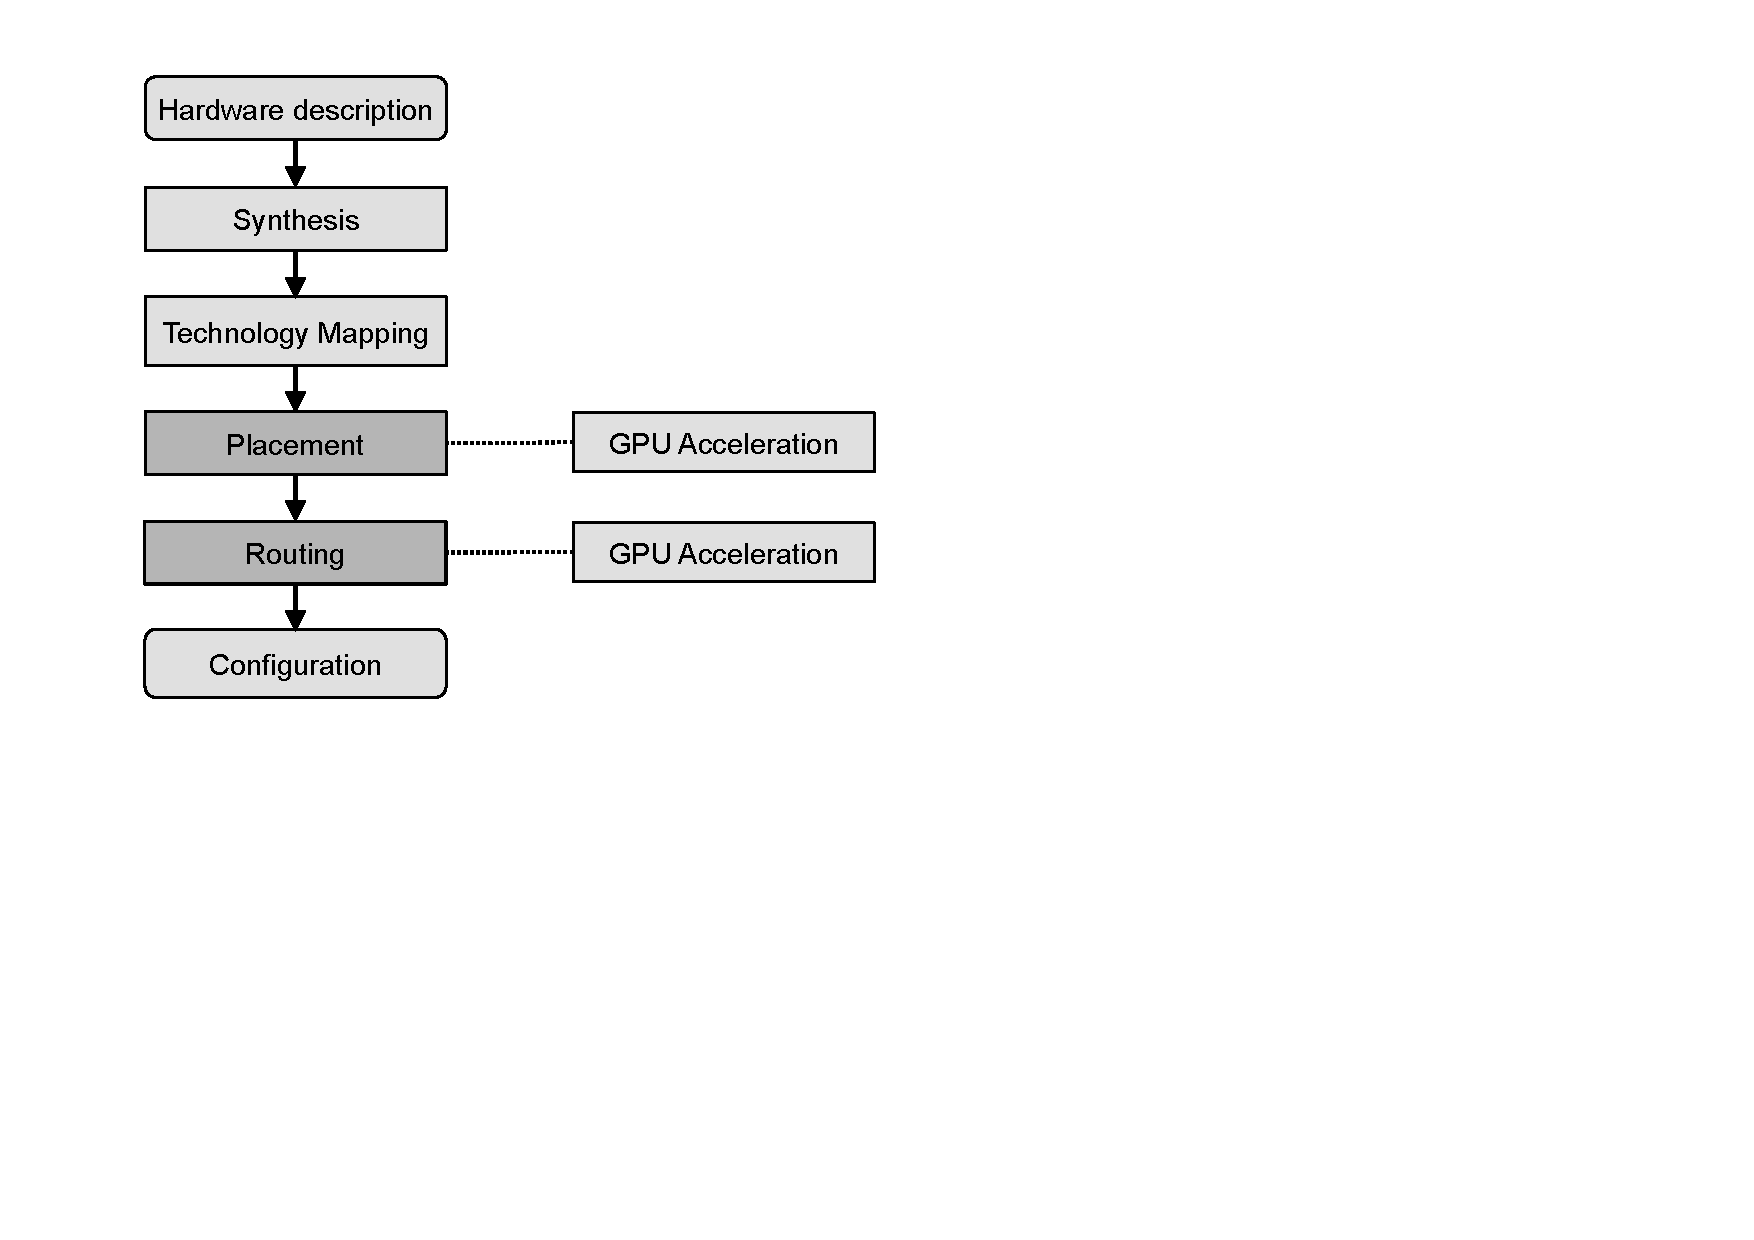
\includegraphics[width = 0.50\textwidth,trim = 0mm 90mm 140mm 2mm, clip]{toolflow}
\caption{Schematic representation of the toolflow. The placement and routing step will be accelerated by a GPU kernel.}
\label{toolflow}
\end{figure}

\begin{figure}[ht]
\centering
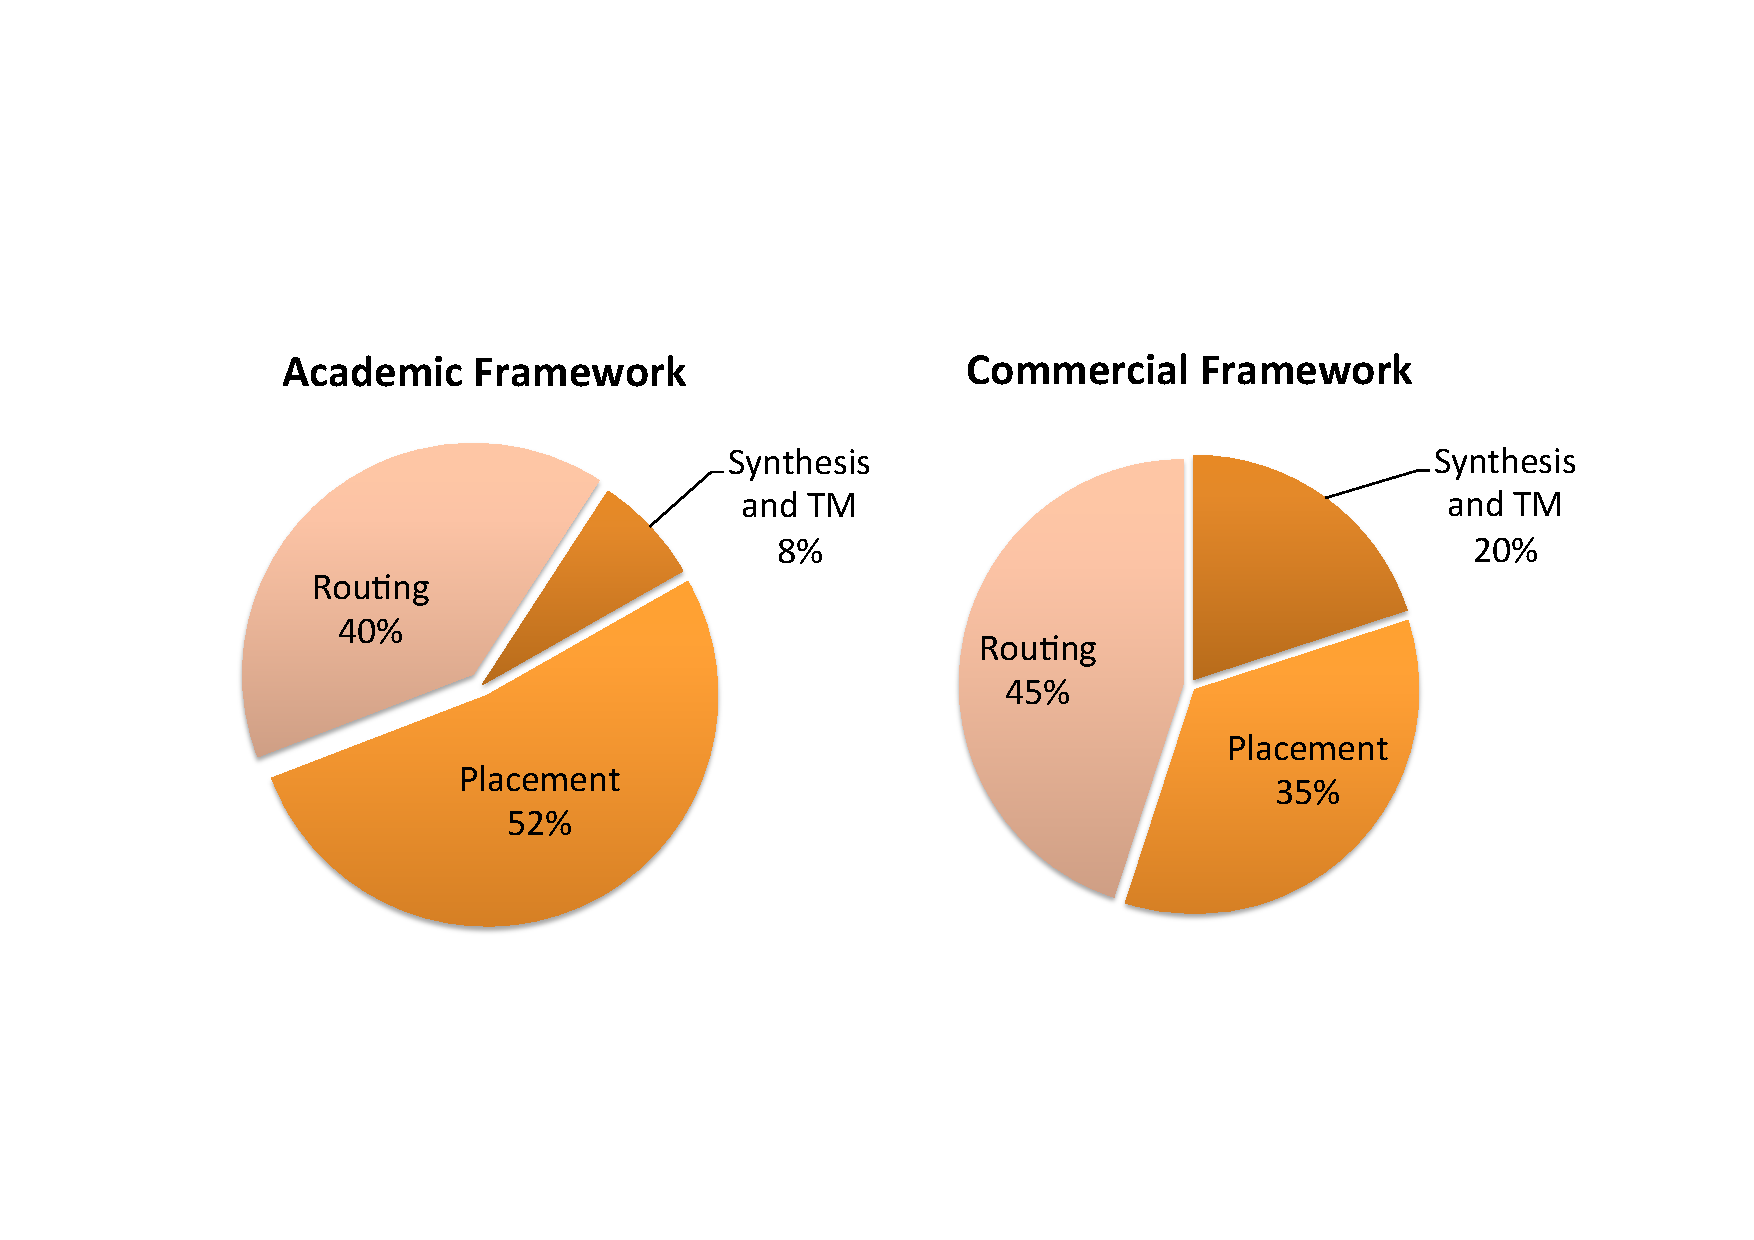
\includegraphics[width = 0.75\textwidth,trim = 0mm 50mm 0mm 40mm, clip]{runtime_breakdown}
\caption{Breakdown per tool of the compilation runtime.}
\label{toolflows}
\end{figure}

\subsection{Placement techniques}\label{placetech}


\subsection{Routing techniques}\label{routetech}

\hl{Routing resource graph
graph based
move away from graph based routing algorithms
tile based
divide and conquer}

\newpage

\section{Timetable \hl{(1 page)}}\label{timetable}
\hl{ Indicate the timeframe for each broad stage considering literature surveys, data collection, production, modelling, review, analysis,
testing, reporting, chapter and thesis writing, and thesis submission date.}

The research in this project will be divided in 2 big stages:

\subsection{Work Packages}
\begin{description*}
\item[Hardware Acceleration of the placement (20 months)]\

\begin{description*}
\item[Adapt the liquid placement algorithm for wide-scale parallelization (9+1 months)]\
In the first step the placer prototype will be further developed and elaborated with the features that were described in the previous section. After this work there is one month allocated for writing a conference paper to report about the initial results.
\item[Implementation of GPU Accelerator for Placement (9+1 months)]\
\\After developing the placement algorithm, it will be implemented on the GPU. Measurements and results will be reported in another conference paper and a demonstration will be held at one of the workshops accompanying a conference. 
\end{description*}

\item[Hardware Acceleration of the the routing (17 months)]\

\begin{description*}
\item[Exploration new routing algorithms for wide-scale parallelization (8 months)] 
Exploring different routing algorithms and devising new algorithms with wide-scale parallelisation in mind. After exploration, the prototype will be implemented and tested. The results will be reported in a conference publication.
\item[Implementation of GPU/FPGA accelerator for Routing (9+1 months)]
After developing the routing algorithm, it will be implemented on the GPU/FPGA. Measurements and results will be reported in another conference paper and a demonstration will be held at one of the workshops accompanying a conference. 
\end{description*}

\item[Writing the doctoral thesis and reporting final results. (6 months)] This time is allocated to write the thesis and to report the finalized results in journals and conferences.  

\end{description*}

\begin{figure}[ht]
\centering
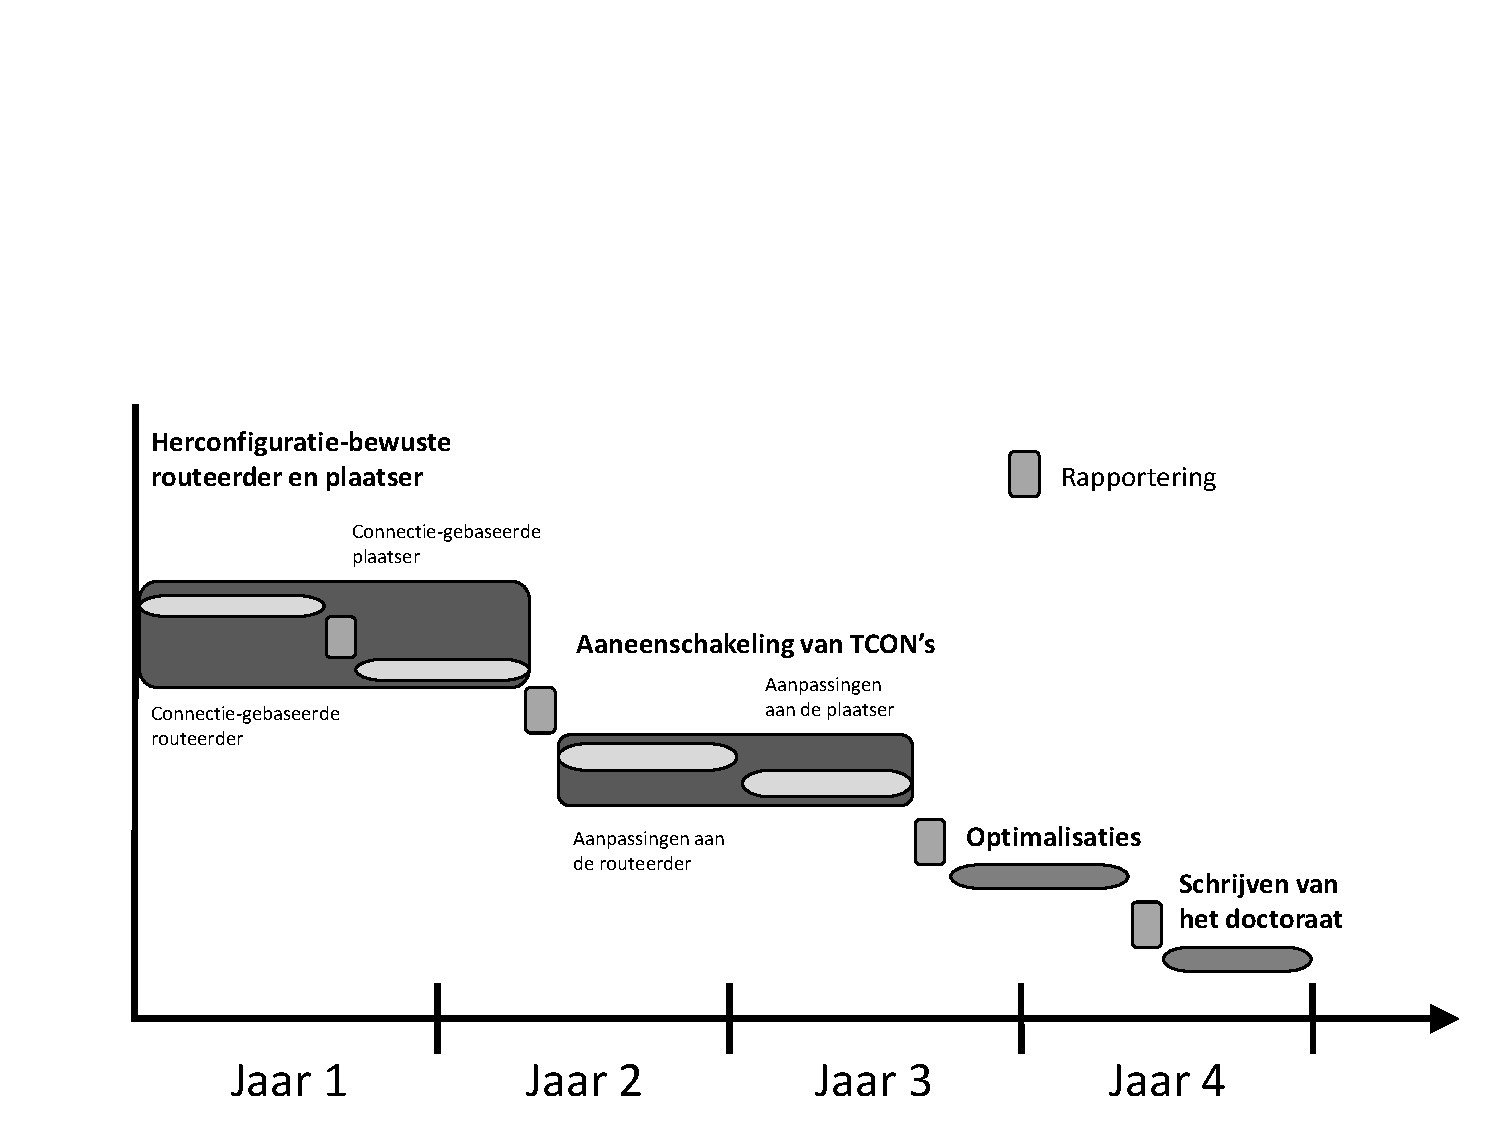
\includegraphics[width = \textwidth,trim = 0mm 0mm 0mm 70mm, clip]{tijdschema.pdf}
\end{figure}

\newpage
\section{Feasibility\hl{(1 page)}}
\hl{Expected outcomes, significance or rationale
Why is it important? 
What do you expect it will deliver? 
What are the expected outcomes? 
Establish the importance of your project by highlighting its originality or why it is worth pursuing. Highlight the benefits, positive expected outcomes or innovative applications of knowledge.}

\hl{Dirk: I can probably write this part after the rest of the proposal is written.\\
Elias: Maybe we can tell here that the first stage is less risk and we are more confident that we will succeed here, because we already developed a good base algorithm that will be easier to parallelize, but for the second stage we did not yet devise a new algorithm. So the second stage has inherent more risk because we have yet to start research there.
@Yun: Can you make a figure for the planning?}


\subsection{Context and Strategy}\label{context}
My research will be conducted at Ghent University in the research group Hardware and Embedded Systems (HES). HES is part of the Computer Systems Lab (CSL) in the Department of Electronics and Information Systems. The HES group is lead by professor Dirk Stroobandt. The group has a lot of experience with developping FPGA CAD tool software.



\newpage
%\nocite{*}
\bibliographystyle{phdsymp}
\bibliography{proposal} % commented if *.bbl file included, as
%\bibliography{../../../bib/hes} % commented if *.bbl file included, as
%%%%%see below
%%DIrk_bis: in je referenties hoofdletters escapen door ze tussen {} te zetten, zoals voor {FPGA}'s.

%%%%%%%%%%%%%%%%% BIBLIOGRAPHY IN THE LaTeX file !!!!! %%%%%%%%%%%%%%%%%%%%%%%%
%% This is nothing else than the phdsymp_sample2e.bbl file that you would%%
%% obtain with BibTeX: you do not need to send around the *.bbl file        
%%
%%---------------------------------------------------------------------------%%
%
%\begin{thebibliography}{1}
%\bibitem{LaTeX}
%Leslie Lamport,
%\newblock {\em A Document Preparation System: \LaTeX, User's Guide and
%  Reference Manual},
%\newblock Addison Wesley Publishing Company, 1986.
%\bibitem{LaTeXD}
%Helmut Kopka,
%\newblock {\em \LaTeX, eine Einf\"uhrung},
%\newblock Addison-Wesley, 1989.
%\bibitem{TeX}
%D.K. Knuth,
%\newblock {\em The {\rm T\kern-.1667em\lower.7ex\hbox{E}\kern-.125emX}book},
%\newblock Addison-Wesley, 1989.
%\bibitem{METAFONT}
%D.E. Knuth,
%\newblock {\em The {\rm METAFONT}book},
%\newblock Addison Wesley Publishing Company, 1986.
%\end{thebibliography}
%
%%---------------------------------------------------------------------------%%

\end{document}

%%%%%%%%%%%%%%%%%%%%%  End of phdsymp_sample2e.tex  %%%%%%%%%%%%%%%%%%%%%%%%%%%

